\documentclass{beamer}
\setbeamertemplate{navigation symbols}{}
\setbeameroption{hide notes}
% To print notes on a second screen or in a notes version, enable:
% \setbeameroption{show notes on second screen=right}

\usetheme{Madrid}
\useoutertheme{shadow}
\useinnertheme[shadow=true]{rounded}
\usepackage{ragged2e}
\usepackage{booktabs}
\usepackage{tikz}
\usepackage{pgfplots}
\usepackage{array}
\usepackage{graphicx}
\usetikzlibrary{arrows.meta,positioning,shapes.geometric}
\pgfplotsset{compat=1.18}

\title[Fraud Detection in ERP Transactions]{Fraud and Abnormal Order Detection in Supply Chain ERP Transactions}
\author{Varad Dharmadhikari \\ Reg. No. 190911xxx \\ Information Technology}
\institute{School of Computer Engineering \\ Manipal Institute of Technology, MAHE}
\date{April 2026}

\logo{
  \IfFileExists{mulogo3.png}{
    \hspace{\dimexpr\paperwidth-1.75cm-5pt}
    \includegraphics[width=1cm,height=1cm,keepaspectratio]{mulogo3.png}
  }{}
}

\setbeamertemplate{footline}[frame number]

\tikzstyle{box} = [rectangle, rounded corners, draw=black, thick, minimum width=1.8cm, minimum height=0.8cm, align=center, fill=blue!10]
\tikzstyle{decision} = [diamond, aspect=2, draw=black, thick, align=center, fill=yellow!15, inner sep=1pt]
\tikzstyle{store} = [rectangle, draw=black, thick, minimum width=2cm, minimum height=0.8cm, align=center, fill=green!12]
\tikzstyle{arr} = [-{Latex[length=2.5mm]}, thick]

\begin{document}

\begin{frame}
\begin{center}
\begin{block}{}
\centering
\large{\textbf{Fraud and Abnormal Order Detection in Supply Chain ERP Transactions}}
\end{block}
\normalsize{\textit{Project Progress Presentation}} \\
\vspace{0.25cm}
\normalsize{\textbf{Varad Dharmadhikari}}\\
\normalsize{Registration Number: 190911xxx} \\
\normalsize{Branch: Information Technology}\\
\vspace{0.6cm}
\textit{\normalsize Under the guidance of} \\
\vspace{0.2cm}
\normalsize{\textbf{Ms. Ramyashree}} \hspace{3.5cm} \normalsize{\textbf{Dr. ABC}}\\
\scriptsize{Internal Guide} \hspace{5.2cm} \scriptsize{External Guide} \\
\vspace{0.5cm}
\scriptsize{\textbf{April 2026}}
\end{center}
\note{
\textbf{Suggested duration: 45--60 seconds.}

\textbf{Presentation points:}
\begin{itemize}
    \item Introduce yourself, the project title, and the fact that this is a progress presentation.
    \item Mention that the project focuses on detecting suspicious ERP-style supply chain orders using machine learning.
    \item Briefly state that the work includes both local execution and Azure-enabled deployment.
\end{itemize}

\textbf{Possible question: Why did you choose this topic?}

\textbf{Answer:} I chose this topic because fraud and abnormal transaction detection is a practical and high-impact problem in ERP and supply chain systems. It also allowed me to combine machine learning, backend development, frontend integration, and cloud deployment in a single end-to-end project.
}
\end{frame}

\begin{frame}
\frametitle{Presentation Outline}
\begin{enumerate}
    \item Introduction and motivation
    \item Literature survey and research gap
    \item Problem definition
    \item Objectives
    \item Methodology and architecture
    \item Work done so far
    \item Results and observations
    \item Remaining work and scope
    \item Conclusion
    \item References
\end{enumerate}
\note{
\textbf{Suggested duration: 30 seconds.}

\textbf{Presentation points:}
\begin{itemize}
    \item Briefly walk the audience through the order of the presentation.
    \item Signal that the presentation will move from motivation, to implementation, to results, to future work.
\end{itemize}

\textbf{Possible question: Is this a research-heavy presentation or implementation-heavy presentation?}

\textbf{Answer:} It is both. I begin with the research context and literature gap, then show the implemented system, current experimental results, and the remaining steps needed to complete the research.
}
\end{frame}

\begin{frame}
\frametitle{Introduction and Motivation}
\begin{itemize}
    \item ERP and supply chain systems process large volumes of orders, refunds, returns, and shipping transactions.
    \item Fraudulent or abnormal behavior is often hidden inside otherwise legitimate-looking records.
    \item Manual review is slow, inconsistent, and difficult to scale.
    \item Machine learning can help assign fraud risk scores and prioritize suspicious records.
    \item A practical solution must work both locally and in an online cloud environment.
\end{itemize}
\note{
\textbf{Suggested duration: 1 minute.}

\textbf{Presentation points:}
\begin{itemize}
    \item Explain that ERP systems are rich in structured transaction data but difficult to monitor manually.
    \item Give examples such as high refunds, billing-shipping mismatch, unusual discount behavior, and suspicious high-value new-customer orders.
    \item Emphasize that the project aims not only to classify fraud but also to build a usable system.
\end{itemize}

\textbf{Possible question: What do you mean by ``abnormal order''?}

\textbf{Answer:} An abnormal order is not always proven fraud. It is a transaction that differs from expected business behavior and deserves attention. For example, a very high-value order from a newly created account with urgent shipping and manual override may not be fraudulent, but it is suspicious enough to be flagged for review.
}
\end{frame}

\begin{frame}
\frametitle{Literature Survey and Research Gap}
\small
\begin{itemize}
    \item Surveys show major challenges in fraud detection: class imbalance, delayed labels, concept drift, and deployment complexity.
    \item Ensemble methods such as Random Forest are strong baselines for structured tabular fraud data.
    \item Hybrid models such as Autoencoder + Random Forest improve complexity handling but increase implementation cost.
    \item Supply chain fraud studies exist, but fewer works present a full upload-to-prediction-to-cloud pipeline.
\end{itemize}

\vspace{0.2cm}
\textbf{Research gap}
\begin{itemize}
    \item Limited focus on ERP-style supply chain order fraud.
    \item Limited end-to-end deployable academic implementations.
    \item Need for a system that is interpretable, modular, and Azure-compatible.
\end{itemize}
\note{
\textbf{Suggested duration: 1.5 minutes.}

\textbf{Presentation points:}
\begin{itemize}
    \item Mention that I reviewed both fraud surveys and supply-chain-specific fraud literature.
    \item Explain that most prior work is concentrated in credit card fraud, while ERP supply chain order fraud is relatively less explored.
    \item State that my project addresses this by focusing on explainable business features and deployable architecture.
\end{itemize}

\textbf{Possible question: Why did you choose Random Forest instead of a deep learning model?}

\textbf{Answer:} Random Forest is a strong baseline for structured tabular data. It is easier to train, interpret, and deploy in a student project. Deep models can be more powerful in some cases, but they require more tuning, more data, and often reduce explainability. I plan to compare advanced models in future work after establishing the baseline.
}
\end{frame}

\begin{frame}
\frametitle{Problem Definition}
\begin{block}{Research Problem}
Design and implement an accurate, explainable, and cloud-capable machine learning system that detects suspicious ERP-style supply chain transactions from uploaded CSV data.
\end{block}

\begin{columns}[T]
\column{0.48\textwidth}
\textbf{Challenges}
\begin{itemize}
    \item Imbalanced data
    \item Missing or inconsistent values
    \item Mixed numeric and categorical fields
    \item Need for interpretable outputs
\end{itemize}

\column{0.48\textwidth}
\textbf{System requirements}
\begin{itemize}
    \item CSV ingestion
    \item Feature engineering
    \item Web-based prediction
    \item Local + Azure deployment
\end{itemize}
\end{columns}
\note{
\textbf{Suggested duration: 1 minute.}

\textbf{Presentation points:}
\begin{itemize}
    \item Clearly define the problem in one sentence first.
    \item Then explain why the problem is difficult: the data is imbalanced, heterogeneous, and operationally messy.
    \item Finally show that the solution must be both predictive and deployable.
\end{itemize}

\textbf{Possible question: Is your project solving fraud detection or anomaly detection?}

\textbf{Answer:} The current implementation is mainly supervised fraud detection because it uses a labeled target field, \texttt{fraud\_label}. However, the system also addresses abnormal-order detection conceptually because the engineered features capture suspicious behavior patterns that may later support anomaly-detection extensions.
}
\end{frame}

\begin{frame}
\frametitle{Objectives}
\begin{itemize}
    \item Build a fraud detection pipeline for ERP-style supply chain transactions.
    \item Preprocess uploaded CSV files and validate required schema.
    \item Engineer business-interpretable fraud features.
    \item Train a machine learning baseline model for fraud scoring.
    \item Expose prediction through a FastAPI backend and browser frontend.
    \item Support both local machine execution and Azure-based deployment.
    \item Optionally persist outputs in Azure Blob Storage.
\end{itemize}
\note{
\textbf{Suggested duration: 45 seconds.}

\textbf{Presentation points:}
\begin{itemize}
    \item Present the objectives as technical milestones.
    \item Emphasize that the project is not just about the model but about the full working pipeline.
\end{itemize}

\textbf{Possible question: Which objective is the most important?}

\textbf{Answer:} The most important objective is building a dependable end-to-end pipeline where uploaded transaction data can be converted into actionable fraud insights. The model is central, but the surrounding system is what makes it practically useful.
}
\end{frame}

\begin{frame}
\frametitle{Methodology: End-to-End Pipeline}
\centering
\resizebox{0.88\textwidth}{!}{
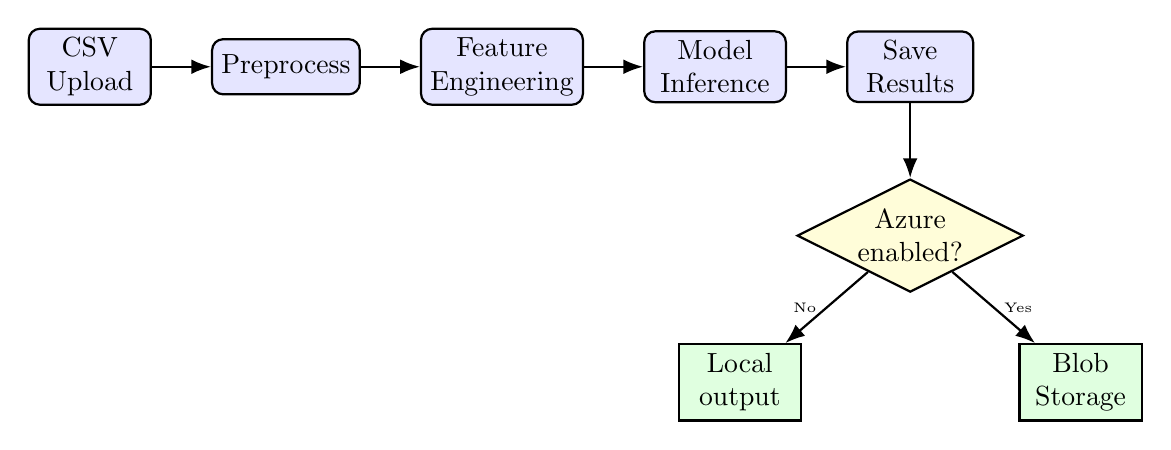
\begin{tikzpicture}[node distance=0.75cm, transform shape]
\node[box, minimum width=1.55cm, minimum height=0.7cm] (upload) {CSV\\Upload};
\node[box, minimum width=1.75cm, minimum height=0.7cm, right=of upload] (prep) {Preprocess};
\node[box, minimum width=1.9cm, minimum height=0.7cm, right=of prep] (feat) {Feature\\Engineering};
\node[box, minimum width=1.8cm, minimum height=0.7cm, right=of feat] (model) {Model\\Inference};
\node[box, minimum width=1.6cm, minimum height=0.7cm, right=of model] (save) {Save\\Results};
\node[decision, below=0.95cm of save, minimum width=1.7cm] (decide) {Azure\\enabled?};
\node[store, below left=1.0cm and 0.65cm of decide, minimum width=1.55cm, minimum height=0.7cm] (local) {Local\\output};
\node[store, below right=1.0cm and 0.65cm of decide, minimum width=1.55cm, minimum height=0.7cm] (blob) {Blob\\Storage};

\draw[arr] (upload) -- (prep);
\draw[arr] (prep) -- (feat);
\draw[arr] (feat) -- (model);
\draw[arr] (model) -- (save);
\draw[arr] (save) -- (decide);
\draw[arr] (decide) -- node[left] {\tiny No} (local);
\draw[arr] (decide) -- node[right] {\tiny Yes} (blob);
\end{tikzpicture}
}

\vspace{0.12cm}
\small
\begin{itemize}
    \item Preprocessing: standardize, validate, deduplicate, impute missing values
    \item Features: mismatch, discount, refund ratio, return ratio, odd-hour behavior
    \item Output: \texttt{fraud\_risk\_score} and \texttt{suspicious\_flag}
\end{itemize}
\note{
\textbf{Suggested duration: 1.5 minutes.}

\textbf{Presentation points:}
\begin{itemize}
    \item Walk through the pipeline from input to output.
    \item Explain that preprocessing cleans the data before model inference.
    \item Explain that the fraud features are business-driven rather than purely statistical.
    \item Mention that after prediction, the output is stored locally and optionally uploaded to Azure Blob Storage.
\end{itemize}

\textbf{Possible question: Why is feature engineering important here?}

\textbf{Answer:} Raw ERP fields alone often do not capture suspicious intent clearly. Feature engineering transforms raw values into fraud-relevant indicators such as shipping mismatch, refund-to-order ratio, and customer return ratio. These features help the model learn business patterns more effectively and also make the output easier to explain.
}
\end{frame}

\begin{frame}
\frametitle{Architecture: Local and Azure Versions}
\begin{columns}[T]
\column{0.48\textwidth}
\textbf{Local machine execution}
\begin{itemize}
    \item Frontend served locally
    \item FastAPI backend at localhost
    \item Model loaded from local \texttt{models/}
    \item Results stored in local \texttt{outputs/}
\end{itemize}

\column{0.48\textwidth}
\textbf{Azure-hosted execution}
\begin{itemize}
    \item Online frontend calls deployed backend
    \item FastAPI hosted on Azure App Service
    \item Storage configured through app settings
    \item Output CSV uploaded to Azure Blob Storage
\end{itemize}
\end{columns}

\vspace{0.3cm}
\begin{center}
\small \textbf{Important note:} only the backend stores the Azure Blob credential; the frontend remains secret-free.
\end{center}
\note{
\textbf{Suggested duration: 1.5 minutes.}

\textbf{Presentation points:}
\begin{itemize}
    \item Compare the two execution modes clearly.
    \item Explain that the local mode is for development and testing.
    \item Explain that the Azure mode is for online access and persistent cloud storage.
    \item Emphasize that the storage secret belongs only in the backend environment, not in the frontend.
\end{itemize}

\textbf{Possible question: Why should the frontend not hold the Blob connection string?}

\textbf{Answer:} The frontend runs in the browser and is visible to the user, so any secret stored there can be exposed. The backend is the correct place for secrets because it runs server-side. In Azure App Service, the connection string or app setting is injected as an environment variable and used securely by the backend.
}
\end{frame}

\begin{frame}
\frametitle{Work Done So Far}
\begin{itemize}
    \item Created synthetic ERP transaction dataset with fraud labels
    \item Implemented preprocessing and validation module
    \item Added engineered fraud features
    \item Trained baseline Random Forest model
    \item Built FastAPI backend with \texttt{/health} and \texttt{/predict}
    \item Built frontend for CSV upload and result display
    \item Added optional Azure Blob upload for generated prediction files
\end{itemize}

\vspace{0.2cm}
\begin{block}{Current project status}
Core end-to-end workflow is functional in local mode and Azure storage support has been integrated.
\end{block}
\note{
\textbf{Suggested duration: 1 minute.}

\textbf{Presentation points:}
\begin{itemize}
    \item Present this slide as a progress checkpoint.
    \item Make it clear that the foundational pipeline is already implemented.
    \item Mention that Azure integration has been added for output persistence.
\end{itemize}

\textbf{Possible question: Which modules are fully complete and which are partial?}

\textbf{Answer:} The dataset generation, preprocessing, feature engineering, model training, backend API, frontend UI, and local output generation are complete. Azure Blob integration is functional, but the production-level user feedback and monitoring around cloud upload can still be improved.
}
\end{frame}

\begin{frame}
\frametitle{Current Results}
\begin{columns}[T]
\column{0.48\textwidth}
\small
\begin{table}
\centering
\begin{tabular}{lc}
\toprule
\textbf{Metric} & \textbf{Value} \\
\midrule
Accuracy & 0.9050 \\
Precision & 0.5000 \\
Recall & 0.0526 \\
F1-score & 0.0952 \\
ROC-AUC & 0.9331 \\
\bottomrule
\end{tabular}
\end{table}

\column{0.48\textwidth}
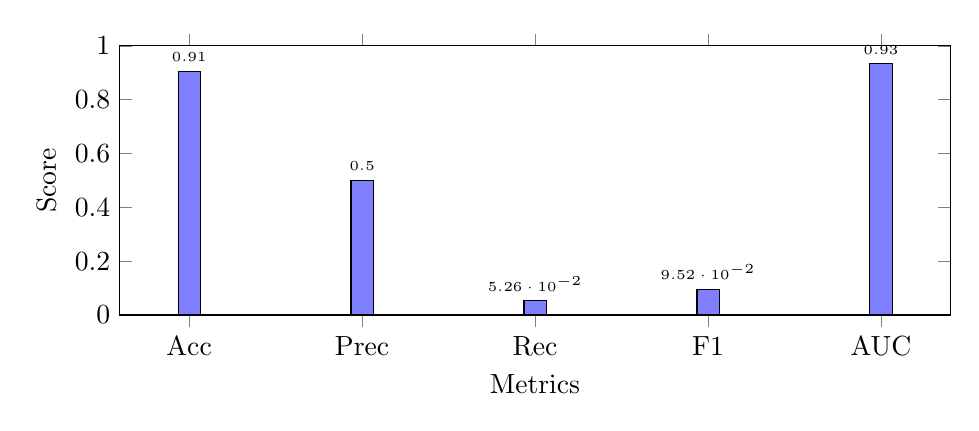
\begin{tikzpicture}
\begin{axis}[
    ybar,
    width=\linewidth,
    height=5cm,
    ymin=0,
    ymax=1,
    bar width=8pt,
    symbolic x coords={Acc,Prec,Rec,F1,AUC},
    xtick=data,
    nodes near coords,
    every node near coord/.append style={font=\tiny},
    ylabel={Score},
    xlabel={Metrics}
]
\addplot[fill=blue!50] coordinates {
    (Acc,0.9050)
    (Prec,0.5000)
    (Rec,0.0526)
    (F1,0.0952)
    (AUC,0.9331)
};
\end{axis}
\end{tikzpicture}
\end{columns}

\vspace{0.2cm}
\small
\begin{itemize}
    \item Total rows: 1000
    \item Fraud-positive rows: 97
    \item Suspicious rows flagged in full pipeline: 80
\end{itemize}
\note{
\textbf{Suggested duration: 1.5 minutes.}

\textbf{Presentation points:}
\begin{itemize}
    \item State the metric values clearly.
    \item Highlight that ROC-AUC is strong, indicating good ranking ability.
    \item Also point out honestly that recall is low, which means the current threshold misses many fraud cases.
    \item Mention that the dataset is synthetic, so these results validate the pipeline but do not yet prove real-world generalization.
\end{itemize}

\textbf{Possible question: Why is accuracy high but recall low?}

\textbf{Answer:} This is because the dataset is imbalanced and the default decision threshold is conservative. The model correctly classifies many legitimate records, which keeps accuracy high, but it identifies only a small fraction of the actual fraud cases, which lowers recall. This is exactly why threshold tuning and imbalance handling are part of the remaining work.
}
\end{frame}

\begin{frame}
\frametitle{Key Observations}
\begin{itemize}
    \item Shipping mismatch, refund-to-order ratio, and customer return ratio are among the most important signals.
    \item The current model ranks risky transactions well, but the decision threshold needs improvement.
    \item The system is already useful as a fraud-screening prototype.
    \item Cloud storage integration makes the solution more deployment-ready.
\end{itemize}

\begin{block}{Main takeaway}
The baseline model is a strong starting point, but performance must be improved especially for recall and operational robustness.
\end{block}
\note{
\textbf{Suggested duration: 1 minute.}

\textbf{Presentation points:}
\begin{itemize}
    \item Interpret the results instead of simply repeating the metrics.
    \item Explain that ranking performance and classification threshold are different issues.
    \item State that the system is already functionally useful as a prototype for analyst support.
\end{itemize}

\textbf{Possible question: How do you know which features are important?}

\textbf{Answer:} I checked the feature importances produced by the Random Forest model. The strongest signals included shipping mismatch, refund-to-order ratio, customer return ratio, order amount, and account age. These are also intuitive from a domain perspective, which increases confidence in the model's behavior.
}
\end{frame}

\begin{frame}
\frametitle{Remaining Work and Scope}
\begin{columns}[T]
\column{0.49\textwidth}
\textbf{Remaining work}
\begin{itemize}
    \item Threshold tuning
    \item Imbalance handling
    \item Model comparison
    \item Cross-validation
    \item Better frontend feedback
    \item Stronger Azure monitoring
\end{itemize}

\column{0.49\textwidth}
\textbf{Scope}
\begin{itemize}
    \item Manufacturing and retail ERP systems
    \item Audit and compliance teams
    \item Supply chain analytics teams
    \item SMEs needing low-cost fraud screening
    \item Academic research and teaching use cases
\end{itemize}
\end{columns}
\note{
\textbf{Suggested duration: 1.25 minutes.}

\textbf{Presentation points:}
\begin{itemize}
    \item Show that the project has a clear completion path.
    \item Emphasize both the technical remaining work and the broader relevance of the project.
\end{itemize}

\textbf{Possible question: What is the most important next step?}

\textbf{Answer:} The most important next step is improving recall while preserving reasonable precision. That means threshold tuning, testing class-imbalance strategies, and comparing the current Random Forest baseline with stronger models such as XGBoost or anomaly-detection methods.
}
\end{frame}

\begin{frame}
\frametitle{Conclusion}
\begin{itemize}
    \item A complete fraud detection pipeline for ERP-style supply chain transactions has been designed and implemented.
    \item The current system supports CSV upload, preprocessing, feature engineering, prediction, result display, and optional Azure Blob upload.
    \item The baseline model shows strong ranking ability but low recall, which defines the next phase of improvement.
    \item The project successfully combines machine learning, software engineering, and cloud deployment.
\end{itemize}
\note{
\textbf{Suggested duration: 1 minute.}

\textbf{Presentation points:}
\begin{itemize}
    \item Summarize what has been achieved.
    \item End by reinforcing that the work is both technically substantial and still evolving.
\end{itemize}

\textbf{Possible question: What is the core contribution of your work?}

\textbf{Answer:} The core contribution is the integration of an explainable fraud-detection pipeline with a usable web architecture that supports both local execution and Azure-based deployment. It is not just a model experiment; it is a complete, working system.
}
\end{frame}

\begin{frame}
\frametitle{References}
\scriptsize
\begin{thebibliography}{10}
\bibitem{r1} Abdallah, A., Maarof, M. A., and Zainal, A., ``Fraud Detection System: A Survey,'' \textit{Journal of Network and Computer Applications}, 2016.
\bibitem{r2} Sorournejad, S. et al., ``A Survey of Credit Card Fraud Detection Techniques,'' arXiv, 2016.
\bibitem{r3} Ahmed, M., Mahmood, A. N., and Islam, M. R., ``A Survey of Anomaly Detection Techniques in Financial Domain,'' \textit{FGCS}, 2016.
\bibitem{r4} Sulaiman, R. B., Schetinin, V., and Sant, P., ``Review of Machine Learning Approach on Credit Card Fraud Detection,'' 2022.
\bibitem{r5} Seify, M. et al., ``Fraud Detection in Supply Chain with Machine Learning,'' \textit{IFAC-PapersOnLine}, 2022.
\end{thebibliography}
\note{
\textbf{Suggested duration: 20--30 seconds.}

\textbf{Presentation points:}
\begin{itemize}
    \item Mention that the work is grounded in fraud-detection surveys, ensemble learning literature, and supply-chain-specific research.
\end{itemize}

\textbf{Possible question: Did you use only academic sources or also official documentation?}

\textbf{Answer:} I used both. Academic sources were used for the research foundation and methodological comparison, while official Azure documentation was used to ensure the deployment and storage setup were technically accurate.
}
\end{frame}

\begin{frame}
\begin{block}{}
\centering
\huge{\textbf{Thank You}}
\end{block}
\vspace{0.3cm}
\centering
\Large Questions and Discussion
\note{
\textbf{Suggested duration: keep for Q\&A.}

\textbf{Common viva questions and detailed answers:}

\textbf{1. Why did you use synthetic data?}

\textbf{Answer:} Real ERP fraud datasets are difficult to obtain due to privacy, access restrictions, and confidentiality. Synthetic data allowed me to create a controlled dataset with meaningful fraud-related patterns so I could validate the system architecture, preprocessing, feature engineering, and baseline model.

\textbf{2. Why is Azure Blob Storage used?}

\textbf{Answer:} Azure Blob Storage is used for persistent cloud storage of generated prediction outputs. It allows the system to store files outside the local machine and supports an online deployment scenario where results can be saved and shared more reliably.

\textbf{3. What are the limitations of the current work?}

\textbf{Answer:} The current limitations are the use of synthetic data, low recall at the default decision threshold, and limited production-level monitoring and security features. These are explicitly identified as part of the remaining work.

\textbf{4. How can the model be improved?}

\textbf{Answer:} The model can be improved through threshold tuning, feature refinement, class imbalance techniques, hyperparameter optimization, and comparison with stronger models such as gradient-boosted trees or anomaly-detection methods.

\textbf{5. Is this solution explainable?}

\textbf{Answer:} Yes, to an extent. The features are business-interpretable and the Random Forest model provides feature importance scores. In future work, SHAP can be added for record-level explanations.
}
\end{frame}

\end{document}
